\chapter{Módszerek}
\pagestyle{headings}

Ebben a fejezetben a teljességre és tömörségre törekedve írom le az alkalmazott módszereket, illetve táblázatosan adom meg a használt anyagok adatait. Abban az esetben, ha a módszer rutinszerű, törekszem rövidített leírásra, és hivatkozom a megfelelő közleményt.

\section{Elektródok}

Munkám során többféle elektródot alkalmaztam. A makroelektródok készítését nem én végeztem, ennek módjáról rövidített leírást adok. A sajátkészítésű mikroelektródok elkészítéséről és jellemzéséről részletesen beszámolok.

\subsection{Szénszál mikroelektród}
Amepox A és B komponensét 1:1 arányban összekevertem, majd egy gyárilag előállított 33 $\upmu$m átmérőjű szénszálat (Specialty Materials Inc. 1449 Middlesex Street Lowell, Massachusetts 01851) a ragasztó segítségével az elektromos elvezetés szigetelő műanyagától elválasztott rézhuzalhoz rögzítettem. A ragasztó megkötéséig szárítószekrénybe helyeztem az elektródokat (kb. 1 óra). Ezután a szénszálat az elektromos elvezetéssel együtt egy húzott végű boroszilikát üvegkapillárisba helyeztem, úgy, hogy a szénszál kb. 5 mm-t lógjon ki a kapillárisból. A kapilláris végének lezárását egy folyékony kétkomponensű epoxi ragasztóval végeztem (helyi barkácsboltból beszerezve), hogy kis mennyiségű folyékony ragasztót a kapilláris végéhez helyeztem, ami a kapilláris hatás miatt a kapillárisba jut, ezáltal egy zárt képezve a kapilláris végén, ami meggátolja a mérendő oldat kapillárisba jutását.
\begin{figure}[h]
\centering
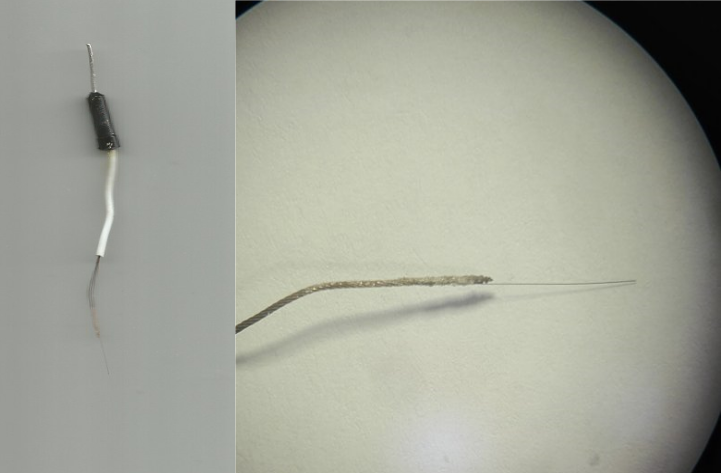
\includegraphics[width=0.5\textwidth]{img/szen33.png}
\caption{(1) Az elektród fotója, ahol (a) elektromos elvezetés, (b) szigetelő műanyagától megfosztott rézhuzal, (c) elektromos vezető epoxi, (d) 33 $\upmu$m átmérőjű szénszál. (2) Az alapelektród mikroszkópikus képe.}
\label{fig:ionophores}
\end{figure}

A 7 $\upmu$m-es szén-mikroelektródot a következőképpen készítettem. Egy elektronikai csatlakozótűbe (,,female pin header'', helyi elektronikai boltban vásárolt) egy 7 $\upmu$m-es szénszálat (Toray Torayca T700S 24K, 19002 50th Avenue East, Tacoma, WA 98446) beleforrasztottam forrasztóón segítségével úgy, hogy a szénszál kb. 1 cm hosszan lógjon ki.A fejléc másik felében egy gyárilag beleforrasztott 1 mm átmérőjű rézdrót volt, amely az elektromos kontaktust biztosítja.
\begin{figure}[h]
\centering
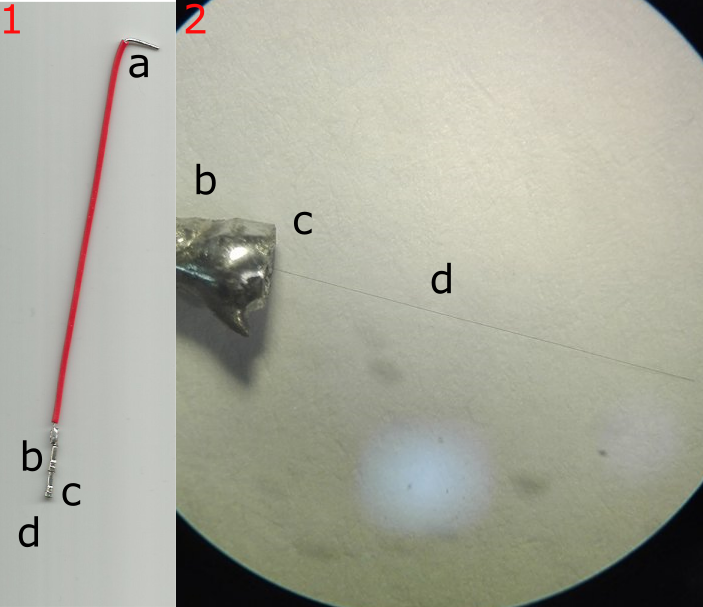
\includegraphics[width=0.5\textwidth]{img/szenmikro.png}
\caption{(1) Az elektród képe látható, ahol (a) elektromos elvezetés, (b) tüskesor csatlakozóalj (female pin--header), (c) forrasztó--ón , (d) 7 $\upmu$m átmérőjű szénszál. (2) Az alapelektród mikroszkópikus képe.}
\label{fig:ionophores}
\end{figure}

%\paragraph{Válaszgyorsaság vizsgálata}

Az oszcilláló reakciók tanulmányozása előtt a mérőműszer válaszgyorsaságát vizsgáltam, hogy biztos legyek benne, hogy elég gyors a kémiai hullámok mérésére. A potenciometriás cella ellenállása és a mérőműszer bemeneti kapacitása együttesen határozza meg az időállandót, mely a cella reagálási sebességét leíró paraméter \cite{kiss2015deconvolution}. A vizsgálatot \emph{,,flip-flop''} típusú 2 V-os 200 ms-os jelgenerátorral végeztem, ami oszcilláló viselkedést mutat. Érdekesség, hogy ez a rendszer ugyanolyan (relaxációs) oszcillátor, mint a vizsgált BZ reakció.

\subsection{Platina mikroelektród}
Gyárilag előállított 25 $\upmu$m átmérőjű platina szálat (Goodfellow Materials) a már jól ismert Amepox A és B komponens 1:1 arányú keverékével ragasztottam egy a szigetelő műanyagától megfosztott elektromos elvezetés réz szálához, amit jól bevált módon kb. 1 órára szárítószekrénybe (100 \textdegree C) helyeztem a kétkomponensű ragasztó megkötéséig.  A megszáradt alapelektródot egy előre kihúzott végű kapillárisba helyeztem, úgy, hogy a platina szál kb. 3-5 mm-re lógjon ki a kihúzott végű kapillárisból. A kapilláris végét folyékony két komponensű ragasztóval zártam le a már fentiekben tárgyalt szénszál mikroelektród készítése alapján. Az elektromos kontaktust ezüst-epoxi (Amepox) biztosította.
\begin{figure}[h]
\centering
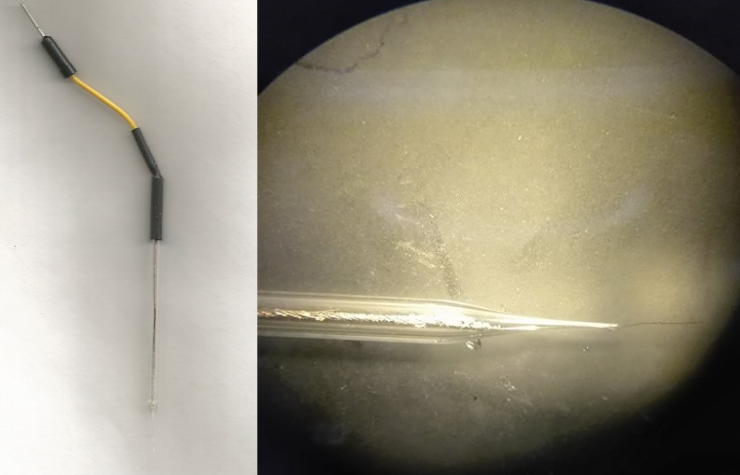
\includegraphics[width=0.5\textwidth]{img/platina.png}
\caption{Az 1-es képen az elektród képe látható, ahol (a) elektromos elvezetés, (b) húzott végű boroszilikát üvegkapilláris, (c) elektromos vezető epoxi, (d) folyadékzár  (e) 25 $\upmu$m átmérőjű platinaszál. A 2-es képen az alapelektród mikroszkópikus képe látható.}
\label{fig:ionophores}
\end{figure}


\section{Oszcilláló reakciók tanulmányozása} 

Minden oszcilláló reakciót a következő eszközök felhasználásával hajtottam végre. Platina vagy szén indikátor elektród és  Ag/AgCl referencia elektródokat használtam. Az alkalmazott szoftver az EDAQ Chart (Doig Ave, Denistone East NSW 2112, Australia) volt. Méréstartományként 1 V-ot alkalmaztam, mintavételezési frekvenciaként 10 Hz-et állítottam be. A mérési adatokat számítógép rögzítette, ami a mérőcellához volt kapcsolva.

\begin{figure}[h!]
\centering
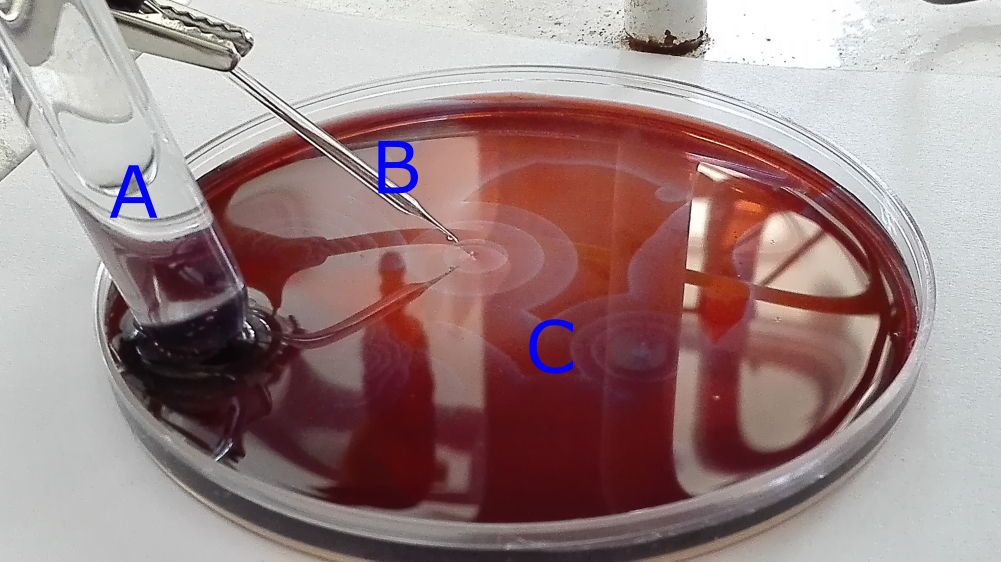
\includegraphics[width=0.5\textwidth]{img/setup.png}
\caption{A mérési elrendezés. (A) Az Ag/AgCl referencia elektród, (B) a mérőelektród, (C) Belouszov-Zsabotyinyszkij reakció Petri-csészében.}
\label{fig:setup}
\end{figure}


\subsection{Makroelektródokkal}

Vizsgálataim során két különböző oszcilláló reakciót tanulmányoztam az általam készített, az előbbiekben említett elektródokkal. 
Először a következő oszcillátor összetételt vizsgáltam \ref{my-label}.
\begin{table}[h!]
\centering
\caption{A reakció komponenseinek koncentrációi.}
\label{my-label}
\begin{tabular}{llllll}
Komponens                       & Malonsav & Kálium-bromát & Kénsav & Mangán-szulfát & Ioncserélt víz \\
\hline
Koncentráció (M)                & 1        & 0.2           & 5      & 0.125          & -              \\
Térfogat (cm$^3$) & 12       & 9             & 11     & 6              & 1              \\
\end{tabular}
\end{table}\\
Ezek a mennyiségek bemérését meghatározott sorrendben végeztem a következőképpen: Először a kétszer ioncserélt vizet mértem be, majd a malonsavat, kálium-bromátot (Reanal Laborvegyszer Kft., Budapest, Magyarország), kénsavat és végezetül a mangán-szulfátot. A reakció a mangán-szulfát hozzáadása után indult. A reakcióelegyet mágneses keverővel kevertem. Ennek a reakciónak a tanulmányozásából messzemenő következtetéseket nem lehet levonni, csak a Field, Noyes és Kőrös által publikált eredmények reprodukálása \cite{noyes1972oscillations} volt a cél, amint azt már a \ref{bromatoszcillator} című fejezetben említettem.

\subsection{Mikroelektródokkal} \label{mikroelektrod}

A Field, Noyes és Kőrös által elért eredmények reprodukálása utána \cite{noyes1972oscillations} keveretlen közegben vizsgáltam a reakciót.
A továbbiakban vizsgált oszcilláló reakciót kevertetés nélkül, a következő összetételű oldatokkal dolgoztam: 

\begin{itemize} \label{komponensek}
\item A oldat: 67 ml H$_2$O + 5 g KBrO$_3$ + 2 ml H$_2$SO$_4$
\item B oldat: 1 g malonsav + 10 ml H$_2$O
\item C oldat: 1 g KBr + 10 ml H$_2$O
\end{itemize}

Az mikroelektródok esetében erősítőt kellett beépíteni az áramkörbe, a terhelési hiba kiküszöbölése végett. 
%A műveleti erősítővel az áramkör kapcsolási rajza az \ref{fig:erosito} ábrán látható. 
A mikroelektródok jelének felerősítése egy TL082-műveleti erősítővel valósult meg a gyakorlatban.

%\begin{figure}
%\centering
%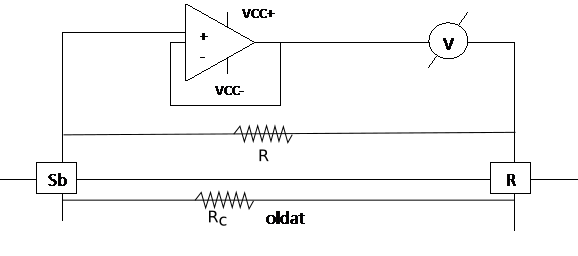
\includegraphics[width=0.8\textwidth]{img/erosito2.png}
%\caption{Feszültségosztó módszer kapcsolási rajza.}
%\label{fig:erosito}
%\end{figure}

\subsection{Pásztázó elektrokémiai mikroszkóp alkalmazása}

\begin{figure}
\centering
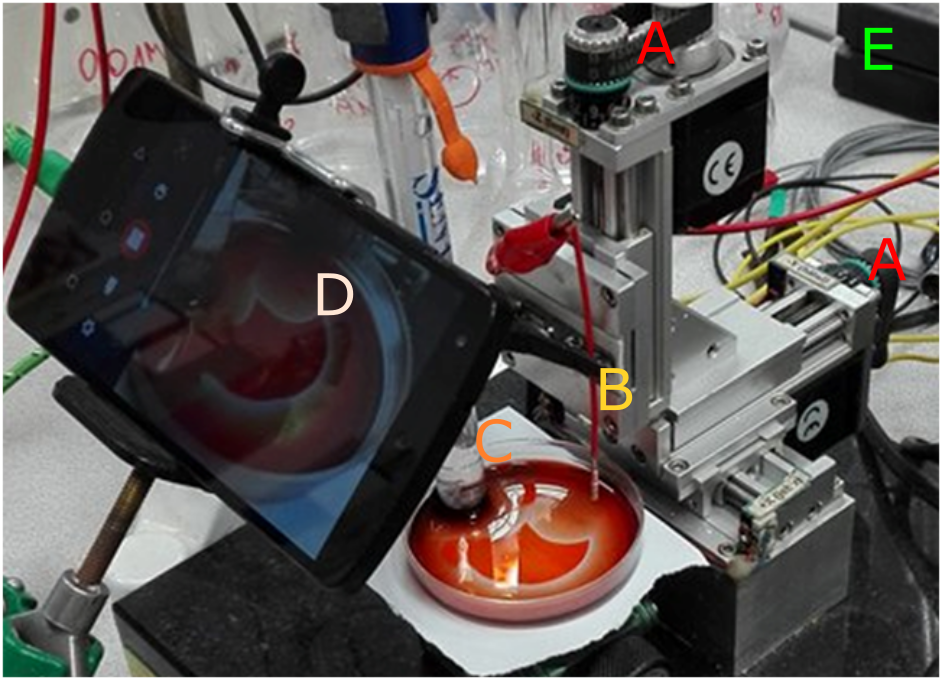
\includegraphics[width=1\textwidth]{img/secm.png}
\caption{Az 1-es képen a mérési elrendezés fotója látható (A) Léptetőmotorok, (B) indikátor elektród (C) referencia elektród, (D) kamera, (E) nagy bemeneti impedanciájú feszültségmérő. A 2-es képen a mérési elrendezés látható.}
\label{fig:secm}
\end{figure}

A \ref{fig:secm} ábra 2-es képén a mérési elrendezés látható, ahol az ábrán látszik, hogy az elektród 1 $\upmu$m-re merült bele a vizsgálandó oldatba. Ezt a mikroszkóp finom léptetőmotorjainak segítségével hajtottam végre (1-es kép A pont), úgy hogy 1 $\upmu$m-es lépésközönként közelítettem az elektródot a vizsgálandó oldat felületéhez, közben figyeltem a potenciált. Amikor a potenciálban ugrást véltem felfedezni tudtam, hogy az elektród az oldatba merül.


\section{Optikai tér-idő kép szerkesztése}
\subsection{Pontszerű mérés}
A mikroelektródok sikeres elkészítése, valamint alkalmazása után az elektrokémiai jelhez képet rendelhetünk, ezáltal megkapva az adott pont elektrokémiai képét, amit következőképpen csináltam. A mérésről videót (8MP Sony Exmor IMX179 1/3,2 inch CMOS szenzor, LG Nexus 5 típusú mobiltelefon) készítettem, amit a pásztázási vonaltól 10 cm-re helyeztem el és 45$^0$-os szöget zárt be azzal. A mikroszkóp által a potenciometriás mikroelektród 500 $\upmu$m/s sebességgel haladt a felületen, 100 $\upmu$m lépésközzel, 10 mm pásztázási úton. A mérés befejeztével a videót a ,,Blender'' \cite{blender} nevezetű program segítségével képkockákra bontottam. A mikroelektród hegyénél lévő 1 pixel $\times$ 1 pixel-es képkockát a teljes mérés során kivettem. A kivett képkockák száma megegyezik a videó hosszával másodpercben véve.

\begin{equation} 
\textrm{Képkockák száma = Videó hossza(s) * Képkocka/másodperc (fps)}
\end{equation}

A telefon által rögzített videók 29.93 fps-al történt. Elegendő másodpercenként egy képkockát kivenni a videóból, ez a gyakorlatban minden 30. képkocka kivételével valósult meg.
Az általam készített elektrokémiai képhez kb. 550 képkockát használtam fel, majd ezeket egymás mellé helyezve az ,,Imagemagic'' \cite{imagemagick} nevű program segítségével megkapjuk az elektrokémiai képet, ami jól látható a ferroin katalizált BZ-reakció esetében. A kép piros szín a ferroin indikátor redukált-, a kék szín az oxidált formához rendelhető. Az így kapott 1 pixeles képeket egymás mellé helyeztem az idő függvényében, majd vertikálisan kinyújtottam és erre helyeztem rá az elektrokémiai információt.
\subsection{PEKM}
\begin{figure}[h!]
\centering
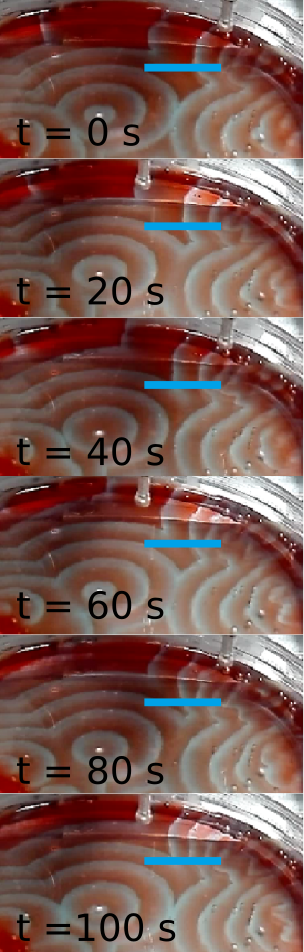
\includegraphics[width=0.3\textwidth]{img/pasztazas.png}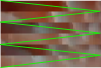
\includegraphics[width=0.3\textwidth]{img/pasztazas2.png}
\caption{Az ábrán látható a mérésről készült videóból kivett képek 20 másodpercenként. Az optikai kép elkészítéséhez a pásztázási szakasznak megfelelő szélességű képet kivettem 1 pixel magasságban (kék vonal az ábrán). A képkockákból kivett részeket (kék vonal) egymásra helyeztem, majd ábrázoltam az idő függvényében. Az ábrán a zöld vonal mutatja az elektród útját a vizsgálat során. Egy vonal mentén zajlott ide-oda a pásztázás, azonban az elektród a tér-idő diagrammon egy cikk-cakk vonalat (zöld vonal) ír le, mivel az idő a mérés során -- természetesen -- halad.}
\label{fig:pasztazas}
\end{figure}

A pontszerű mérés, valamint a PEKM mérés során kapott optikai- és eletrokémiai technika kombinálását az \emph{"Eredmények"} című fejezetben mutatom be.
